\lecture{3}{1. September 2025}{Systems of forces and moments}

\subsection{Moment of a couple}
A \textit{couple} is defined as two parallel forces that hav equal magnitude but opposite directions and are separated by a distance $d$ as shown on \textbf{\autoref{fig:f3_25}}. Since the resultant force of the couple is zero the only effect is to produce a tendency for rotation.

\begin{figure} [ht]
  \centering
  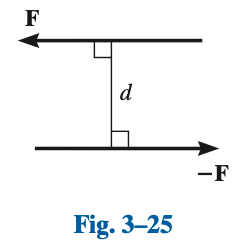
\includegraphics[width=0.25\linewidth]{./figures/f3_25.png}
  \caption{}
  \label{fig:f3_25}
\end{figure}

The moment produced by a couple is called a \textit{couple moment} it can be shown that this is equal to:
\[ 
\textbf{M} = \textbf{r} \cdot \textbf{F}
.\]
This is a \textit{free vector}, i.e. it can act at \textit{any point} since $\textbf{M}$ only depends on the position vector $r$ between the forces and not the position vectors from the origin.


\subsection{Simplification of a force and couple system}
It is often convenient to reduce a complex system of forces and couple moments acting on a body to a simpler form by replacing it with an equivalent system. A system is equivalent if the \textit{external effects} it produces on a body are the same as those caused by the original force and moment system. 

Every system of several forces and couple moments can be broken down into a single resultant force acting at a point $O$ and a resultant couple moment. This can be done by adding together the forces in each Cartesian direction as well as the moments each on their own. 

\subsection{Reduction of a simple distributed loading}
Sometimes, a body is subjected to a load distributed over its surface. The pressure caused by this distributed loading on the surface represents the loading intensity and is measured in \unit{Pa}. 

The most common type of distributed loading is that along a single axis. Take for example a beam of constant width $b$ subjected to a pressure loading that varies along the $x$-axis. The loading is described by the function $p = p(x)$. Since this contains only one variable we can quickly ``one-dimensionalize'' the problem by $w(x) = p(x) b$. 

The magnitude of the resultant force in this case must be found using integration as summing ``all the forces'' would require an infinte sum. I.e.
\[ 
F_R = \int_{L} w(x) \, \mathrm{d}x = \int_A \, \mathrm{d}A = A
.\]
The location $\overline{x}$ of $\textbf{F}_R$ can be determined using static equilibrium and moments as:
\[ 
- \overline{x} F_R = - \int_L x w(x) \, \mathrm{d}x 
.\]
And solving for $\overline{x}$ we have:
\[ 
\overline{x} = \frac{\int_L x w (x) \, \mathrm{d}x}{\int_L w(x) \, \mathrm{d}x} = \frac{\int_A x \, \mathrm{d}A}{\int_A \, \mathrm{d}A}
.\]
